%----------------------------------------------------------------------------------------
%  CHAPTER CONTENTS
%----------------------------------------------------------------------------------------

\chapter*{Identify Factors that Predict Intro CS Experience Based on Gender}

\section*{Project Overview}

One of the biggest challenges at the start of this century is successfully getting people into the technical workforce. We are now in a new technological era with autonomous cars driving down our streets and bots like Alexa and Siri becoming an extension of our lives. As automation continues to gain ground, so too are the new industries it helps to create. This new era is creating a new kind of worker, the highly-skilled knowledge worker, in particular, the highly-skilled \emph{technology} knowledge worker.

This shift in the workforce towards highly skilled, technical knowledge workers poses a challenge on the supply side; mostly because of a lack of presence of computer science in K-12 education; the under-production of post-secondary degrees in computer science;  the underrepresentation of women and/or the underrepresentation of ethnic minorities. One of the solution that has been proffered for this problem is redesigning introductory computer science to broadening participation.  

As part of my doctoral study, I decided to study the socio-curricular factors that affect the decision to participate in introductory computer science through a data-driven lens. To do this, I designed a research study investigating the role of computer science self-identity centered around the experiences of undergraduates in two introductory computer science classes at UC Berkeley. 

The major motivation for doing this project is to gain some insight into what factors most govern the experiences of historically underrepresented students as they enter the CS pipeline at the University level.

If we are able to truly understand indicators that specifically \emph{increase} a \textbf{sense of belonging in CS} for URMs, then we can create environments where these factors abound. Once we have such an environment; we can determine the effect on both male and female students; if we find out that these kinds of environment positively support CS belonging in both groups, we can then make the recommendation that we design our CS learning environments along those lines. The first step in such a scheme would be to determine the salient factors around the gendered experience of CS, which is what this reason why this project exists.


\section*{Problem Statement}

With this project, the problem I am interested in investigating is the gendered experience of the two CS classes in the study. Using machine learning algorithms, I want to identify the leading indicators of the experience of belonging broken down by gender in introductory CS at an elite research university like Berkeley.

To solve this problem, I will follow the following course of action:
\begin{enumerate}% 
\item Explore the dataset.\\
Usually, I would explore the dataset to ensure its integrity and understand the context. But in this case, I will skip this step since I designed the study and collected the data, as such, I am well versed of the context. Further, I have done previous work on this dataset, so I know its boundaries.
\item Identify features that may be used.\\ 
If possible, engineer features that might provide greater discrimination.
\item With the understanding that this a ``classification'' task, explore a couple of classifiers that might be well suited for the problem at hand.
\item Once a classifier has been selected, tune it for optimality.
\end{enumerate}

\section*{Metrics}


Predicting gender in intro CS is a supervised learning problem. To determine the performance of the model, I will be using the $F_1$ score, i.e., the weighted average of precision and recall as our metric of choice. 

I am choosing to use the $F_1$ score as my metric of evaluation over the accuracy score because my particular dataset has more male students in it than female students. You can see this imbalance in figure \ref{targetClass}. If I used accuracy, because this imbalance is there, my results could be misleading. 

Beyond precision and recall, what we will lean on to give us confidence about our model will be taking a look at the confusion matrix that each model generates. This matrix will let us see which model most accurately \emph{identifies female} students. This will be the \textbf{most important} evaluation metric because that is the segment on the student population we are most interested in learning what indicators will point towards a sense of CS belonging.

\begin{figure}[!hbtp]
\centering

    \caption{\textbf{Target Class. }\textit{The histogram shows a slightly unbalanced target dataset with 494 values of \{0: male\} and 388 values of \{1: female\}.}}

    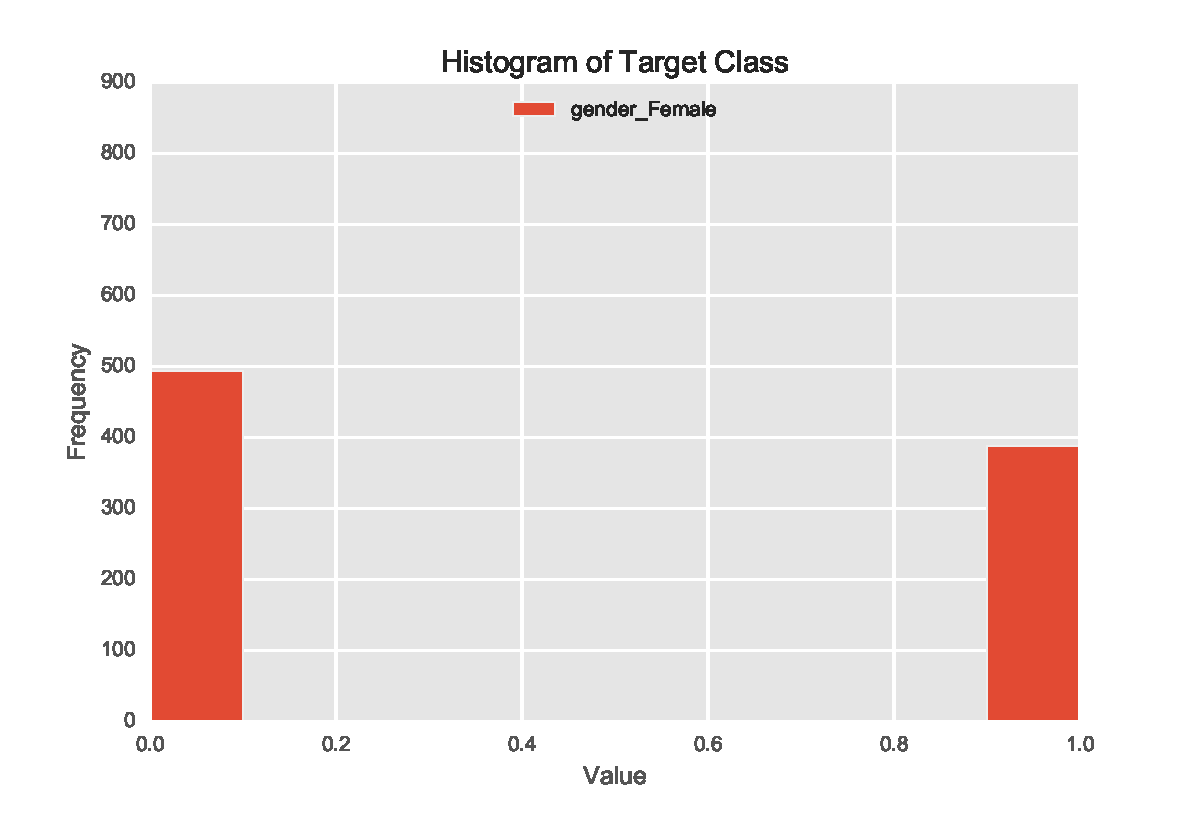
\includegraphics[width=1\textwidth]{figures/targetClass}
    \label{targetClass}
\end{figure}

%----------------------------------------------------------------------------------------
%  CHAPTER 
%----------------------------------------------------------------------------------------

\chapter*{Analysis}

\section* {Dataset}
The dataset used in this project consists of survey responses. A copy of the survey instrument can be found in the appendix of this report. The survey instruments were developed to measure participants' self-reported attitudes along several dimensions: 

\begin{enumerate}% 
\item CS beliefs
\item Gendered belief about CS ability
\item Career driven beliefs about CS
\item Computational thinking beliefs
\item CS belonging
\item Collegiality
\end{enumerate}

In addition, the survey also collected data around student background: 

\begin{enumerate}% 
\item Prior collegiate CS exposure
\item CS mentors and role models
\item University demographics
\end{enumerate}



Majority of the questionnaire uses a 5-point Likert scale (where 1 = Strongly Disagree, 3 = Neutral and 5 = Strongly Agree). A code book was created to facilitate ease of analysis and interpretability of results. The dataset consists of 882 instances with no missing data. Further, there are 494 males and 388 female samples in the dataset. 


\section*{Algorithms and Techniques}

For the problem of predicting gender in intro CS, I experimented with four different classifiers, a decision tree classifier, two ensemble methods and a support vector machine:

\begin{enumerate}% 
\item I selected a Random Forest classifier because it is considered one of the best off-the-shelf learning algorithm, and requires almost no tuning. 

\item Another selection was the eXtreme Gradient Boosted (XGBoost) trees classifier; which is an advanced implementation of the gradient boosting algorithm. From reading literature on machine learning in practice, the XGBoost classifier has differentiated itself as a classifier that has successfully demonstrated its performance in a wide range of problems. For example, ``among the 29 challenge winning solutions published at Kaggle's blog during 2015, 17 solutions used XGBoost.''

\item The Support Vector Machine (SVMs) was selected because they are very robust classifiers and \textit{more importantly}, they have a method to correct for class imbalances. 
              
\item Finally a Decision Tree classifier was also selected. The \textit{major} reason why the decision tree classifier was selected was its interpretability. For this problem domain, it is not just satisfactory to discriminate between male and female students, what I ultimately want is to gain \textit{insights} into what the salient factors around the experience of intro CS are, based on gender.

\end{enumerate}

\section*{Benchmark}

This is novel research, as a result, there are no benchmarks to compare the performance of our classifiers with.


%----------------------------------------------------------------------------------------
%  CHAPTER 
%----------------------------------------------------------------------------------------
\chapter*{Methodology}


\section*{Data Preprocessing}

To prepare the data for classification, all features need to be transformed into numeric data. This dataset has several non-numeric columns that need converting. Many of them take on \texttt{yes} and \texttt{no} values, e.g. \texttt{prcs\_2}. These can be reasonably convert these into `1'/`0' (binary) values. For the columns whose values are `Nan', these will be converted to `0'. Further, spaces will be removed from column names with the understanding that the tree plotting algorithm for Xgboost will fail if column names have spaces. 

The feature were scaled using a minimax scaler to get better output for our SVM. This yielded the following values:
\begin {itemize}
\item Strongly Disagree = 0.0
\item Disagree = 0.2
\item Neutral = 0.6
\item Agree = 0.8
\item Strongly Agree = 1.0
\end{itemize} 



\section*{Frequency Distribution}
We created a frequency distribution for some dimensions in our data to see if there are features that have extremely low spread in their distribution. From figures \ref{atct_dimension}, \ref{atcs_dimension}, and \ref{blg_dimension}, we know that these variables are broadly distributed.

\begin{figure}[!hbtp]
\centering
    \caption{\textbf{Frequency distribution for dimension atcsgender. }\textit{Gendered belief about CS ability.}}\label{atcsgender_dimension}
    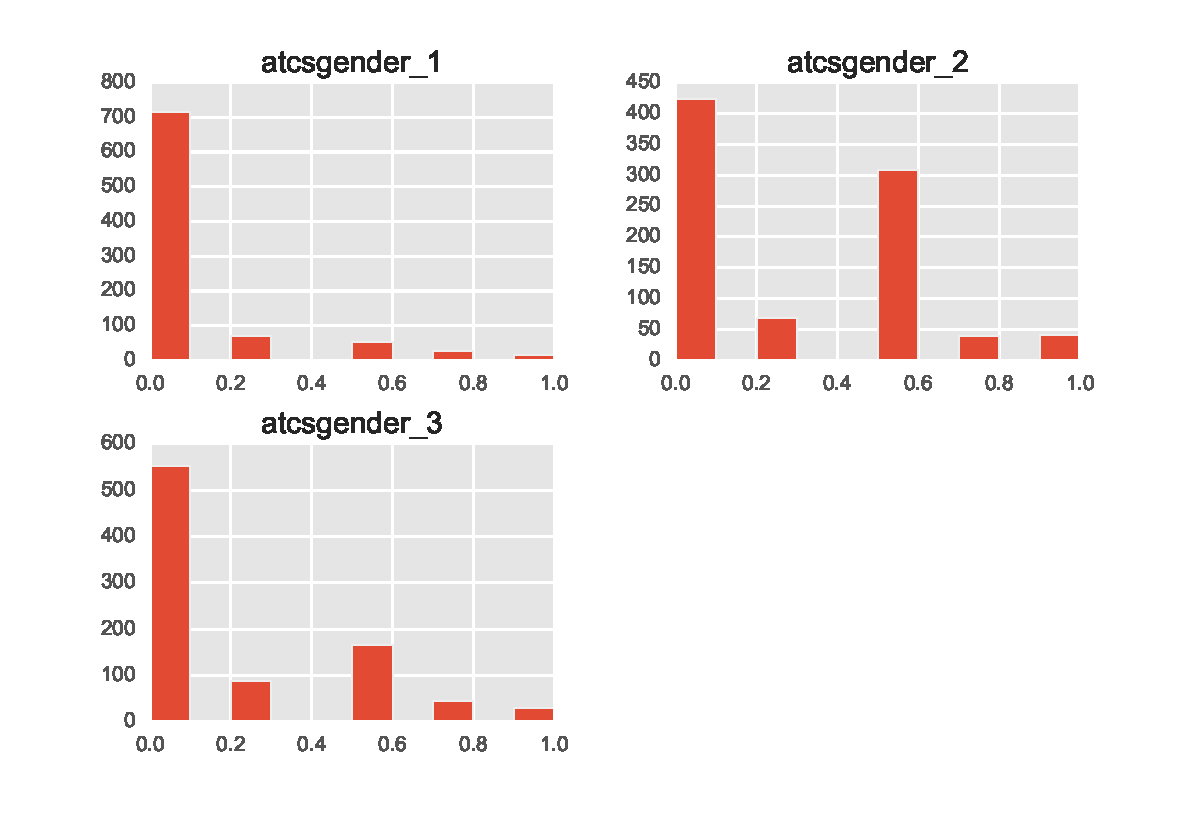
\includegraphics[width=1\textwidth]{figures/atcsgender_dimension}
\end{figure}

\begin{figure}[!hbtp]
\centering
    \caption{\textbf{Frequency distribution for dimension atcs. }\textit{Self-reported attitudes about CS.}}\label{atcs_dimension}
    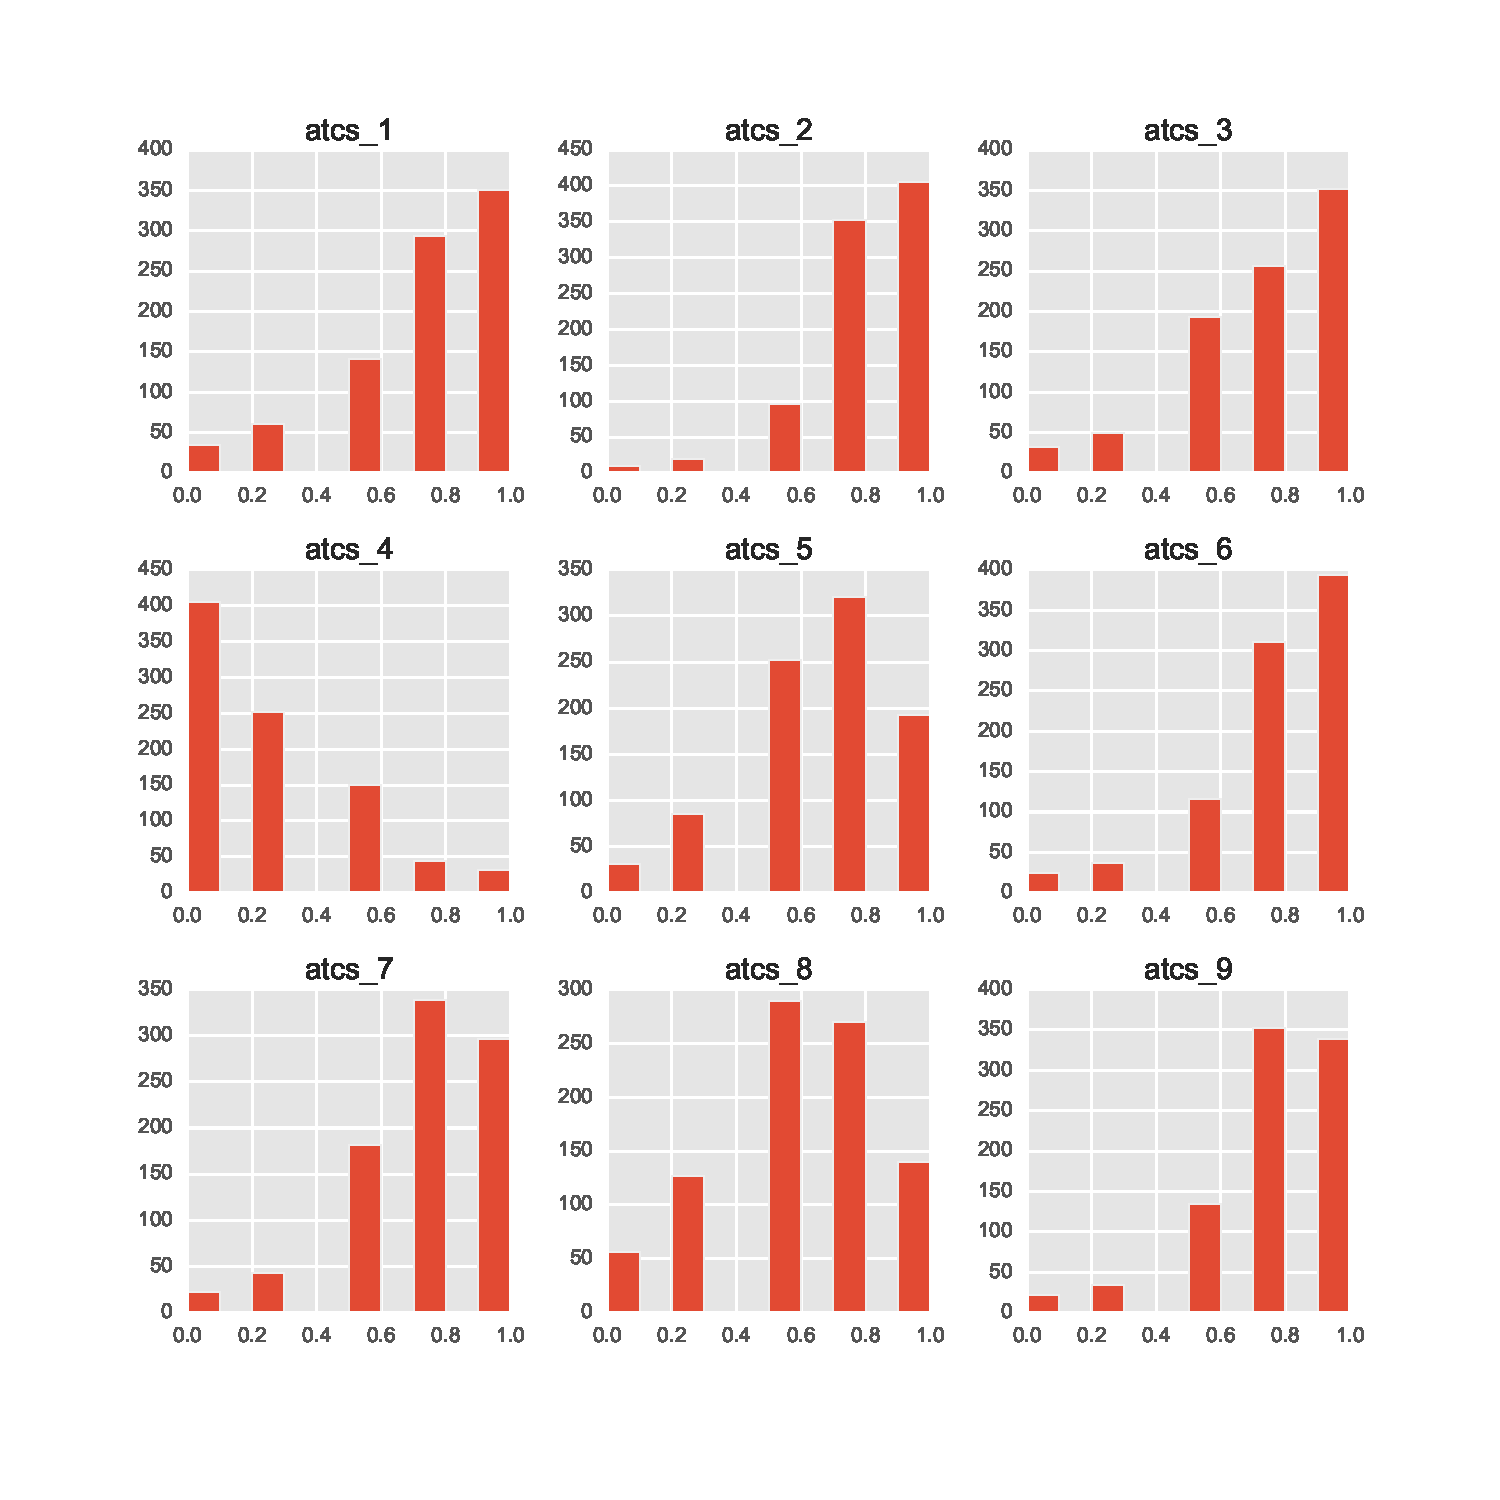
\includegraphics[width=1\textwidth]{figures/atcs_dimension}
\end{figure}

\begin{figure}[!hbtp]
\centering
    \caption{\textbf{Frequency distribution for dimension atct. }\textit{Self-reported attitudes about computational thinking.}}\label{atct_dimension}
    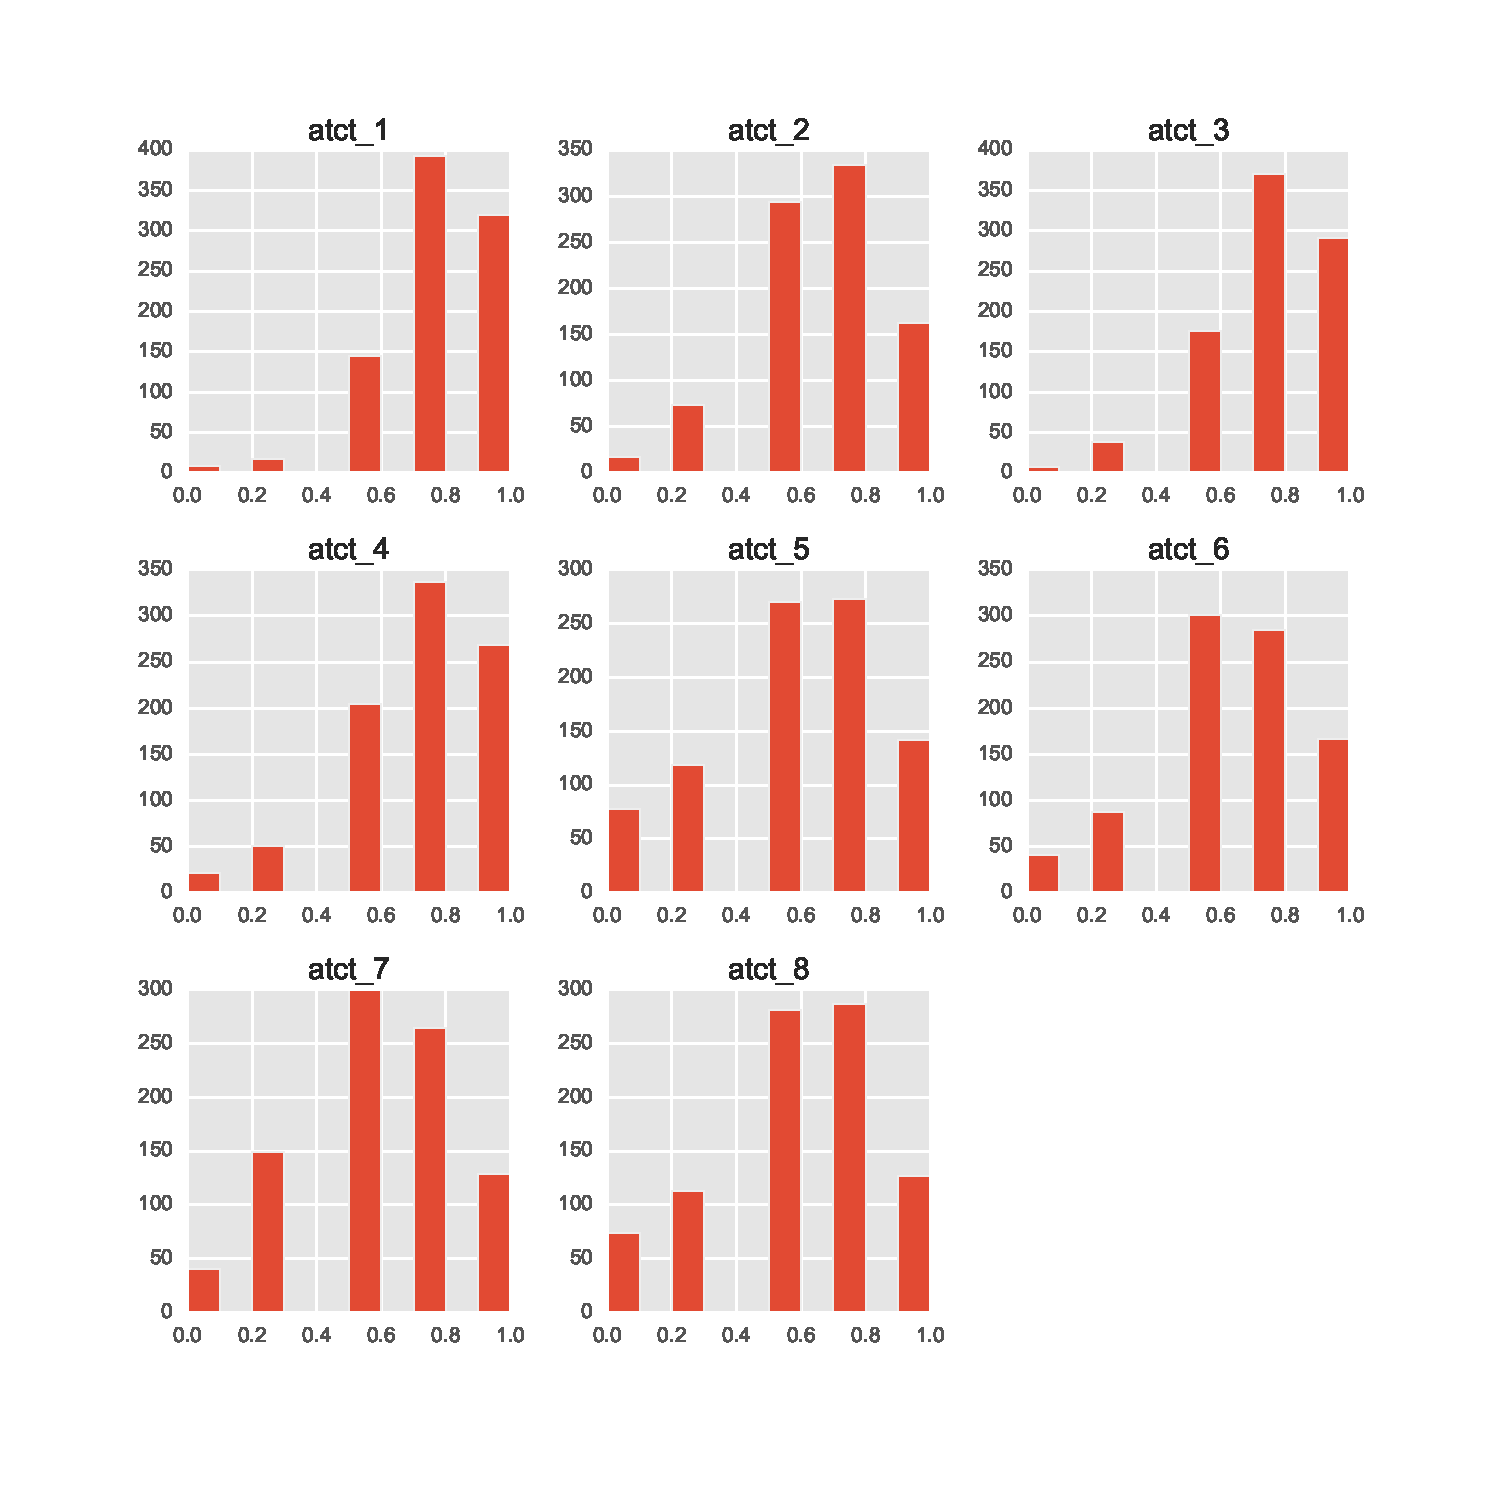
\includegraphics[width=1\textwidth]{figures/atct_dimension}
\end{figure}

\begin{figure}[!hbtp]
\centering
    \caption{\textbf{Frequency distribution for dimension blg. }\textit{Self-reported attitudes about CS class belonging.}}\label{blg_dimension}
    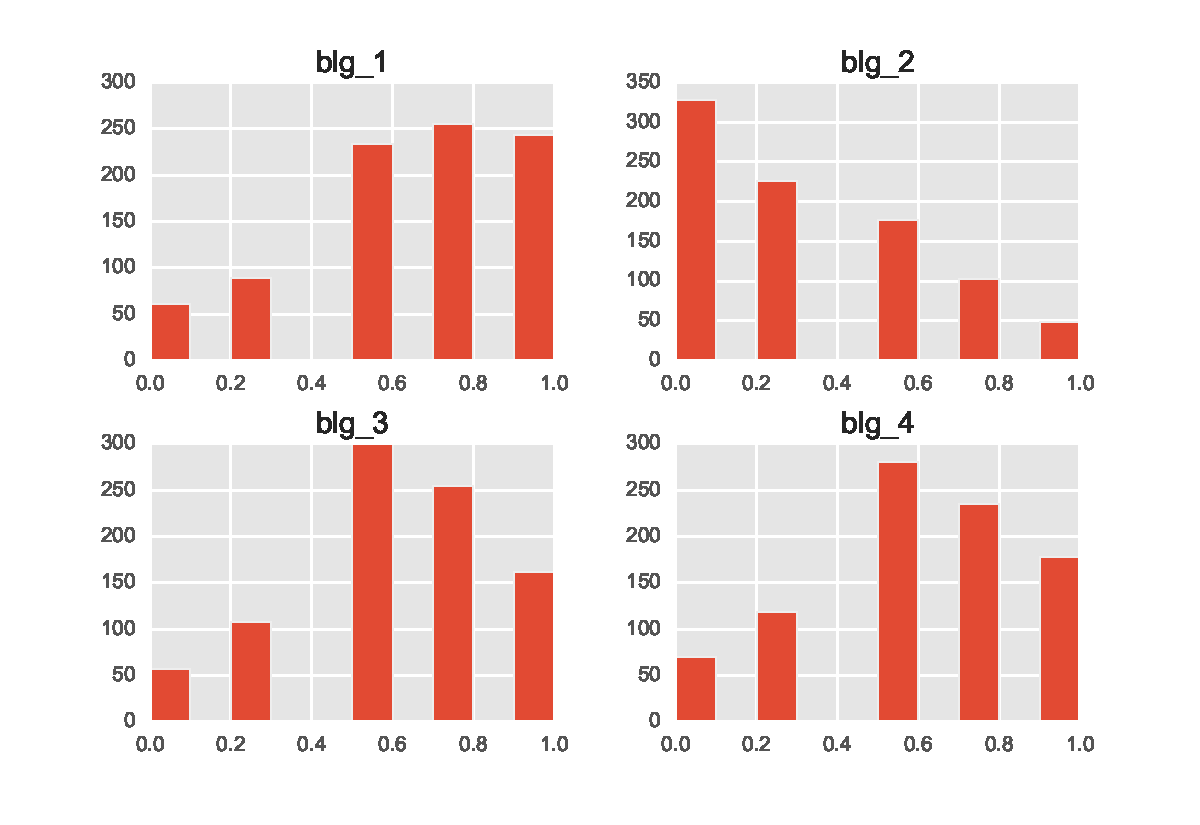
\includegraphics[width=1\textwidth]{figures/blg_dimension}
\end{figure}

From \ref{atcsgender_dimension}, we can see that the distribution for the dimension \texttt{atcsgender} is extremely skewed to the right, further we notice that \texttt{atcsgender\_2} is bimodal. 

In doing these frequency distributions we are trying to gain an understanding of the variables and determine if we need to reject some of them, or collapse other.




\section*{Implementation}
We implemented the four learning algorithms. For each of the learners we implemented the baseline algorithm using a stratified shuffle split cross validation with 50 folds and calculated the $F_1$ scores and looked at the confusion matrices respectively. 


\setlength{\extrarowheight}{1.5pt}
\begin{table}[!htbp]
\caption{Scores} %title of the table
\centering % centering table
\begin{tabular}{|p{6cm}|p{1.5cm}|} % creating four columns
\hline % inserts single-line


\multicolumn{2}{|c|}{}\\
\multicolumn{2}{|c|}{Result of training the baseline classifiers}\\[5pt]
\hline
Classifier & F1 Score\\[0.5ex]
\hline % inserts single-line

SVC     & 0.541\% \\
DecisionTree       & 0.579\% \\
RandomForestClassifier   & 0.608\% \\
XGBClassifier            & 0.693\% \\

\hline% inserts single-line
\end{tabular}
\label{tableBenchMarkScores}
\end{table}

In figure \ref{plot_tree} we see the decision tree for the first two xgboost trees. This figure gives us insight into which features were doing the most work of splitting the data, and consequently may have the largest impact on predicting gender in introductory CS experience.


\begin{figure}[!hbtp]
\centering
    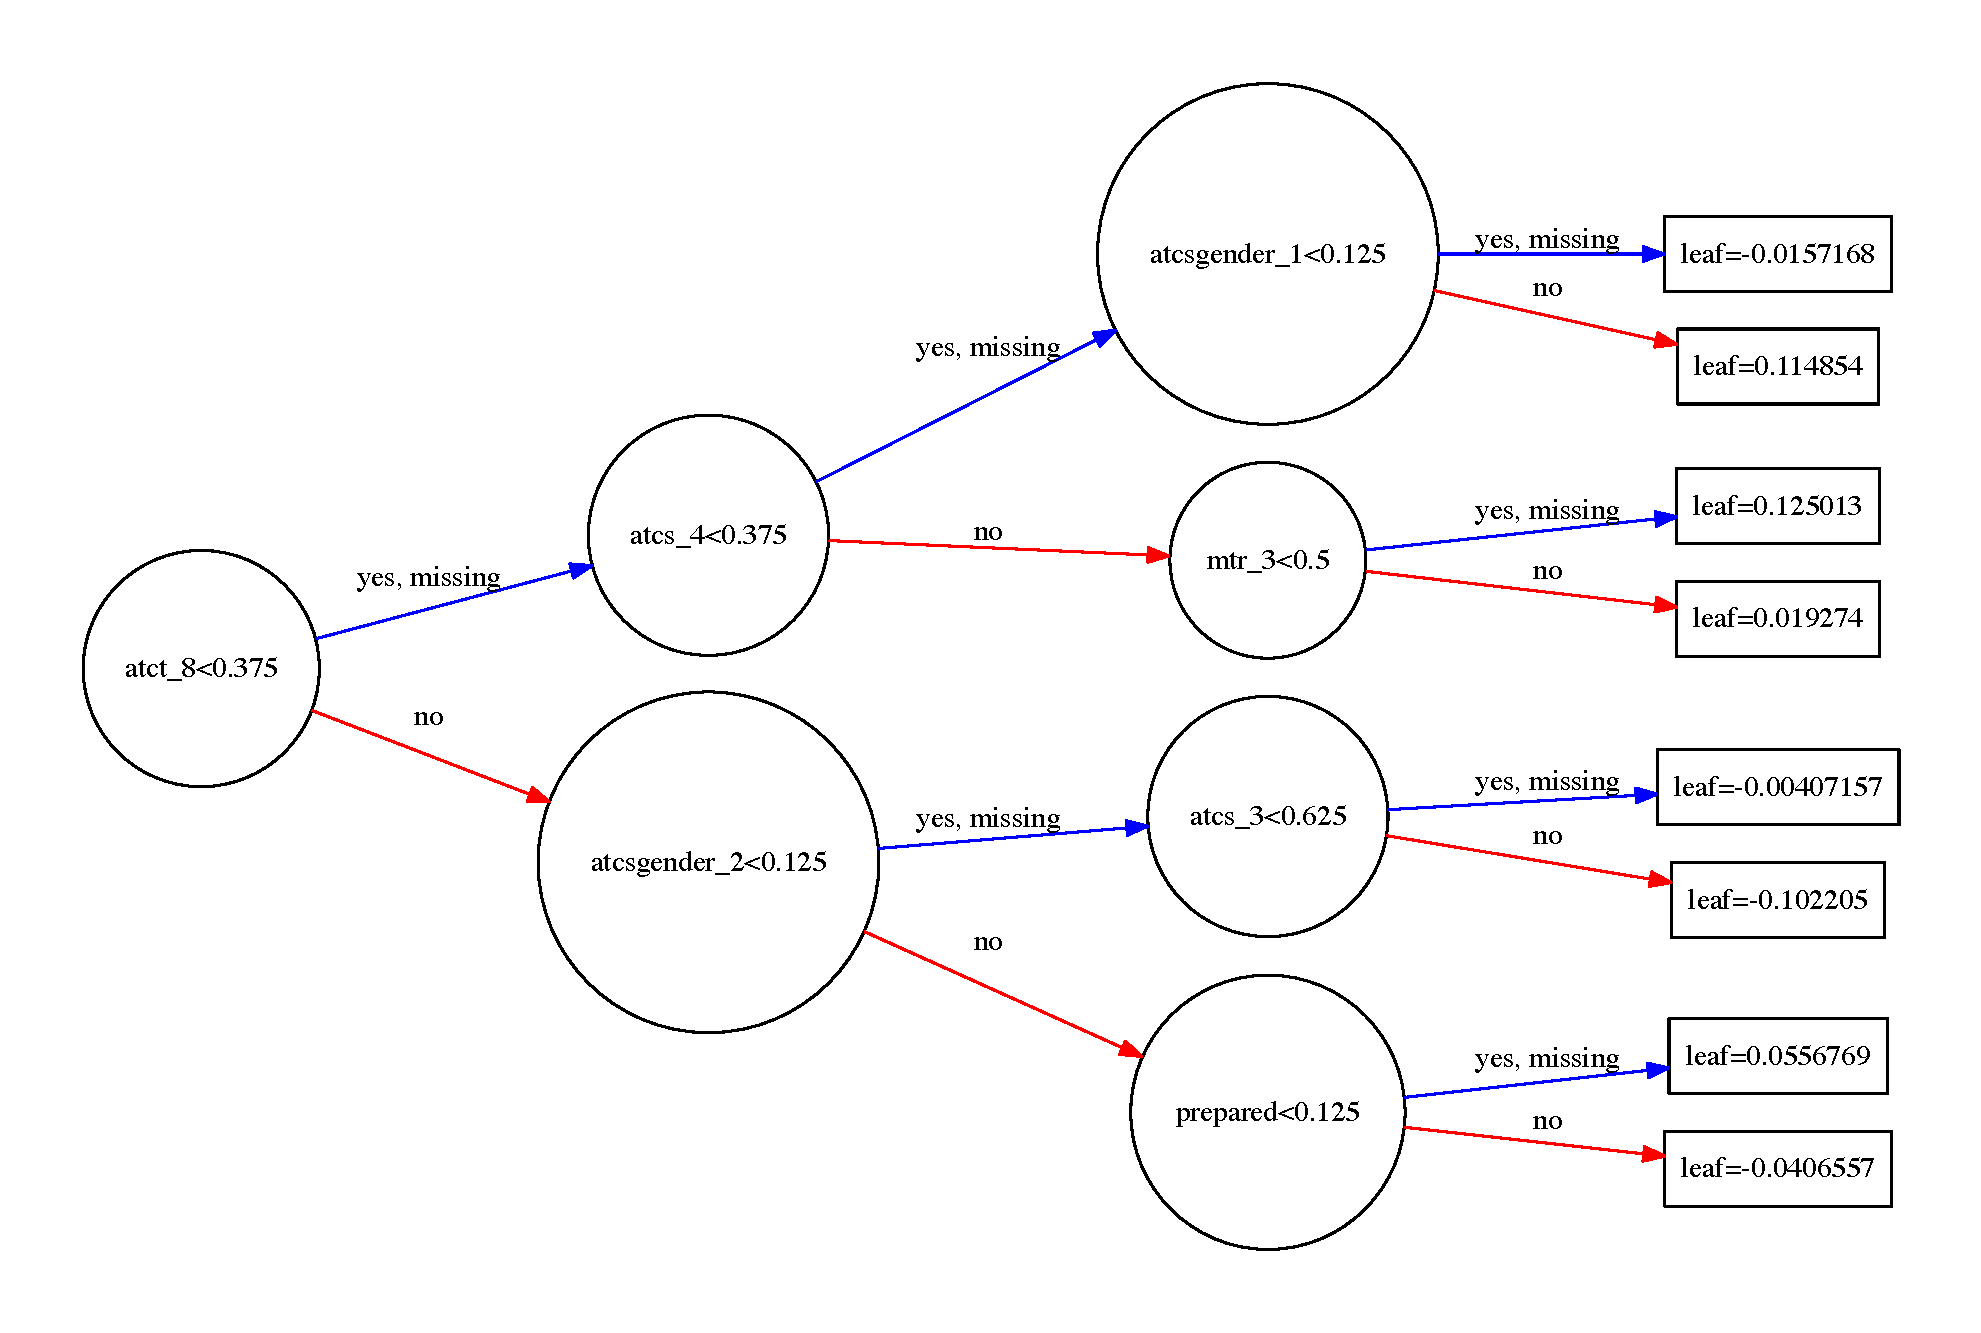
\includegraphics[width=1\textwidth]{figures/X_graph}
    \caption{\textbf{XgBoost estimator decision tree. }\textit{}}\label{plot_tree}
\end{figure}



\begin{figure}[!hbtp]
\centering
    \subfloat[Random Forest]{%
    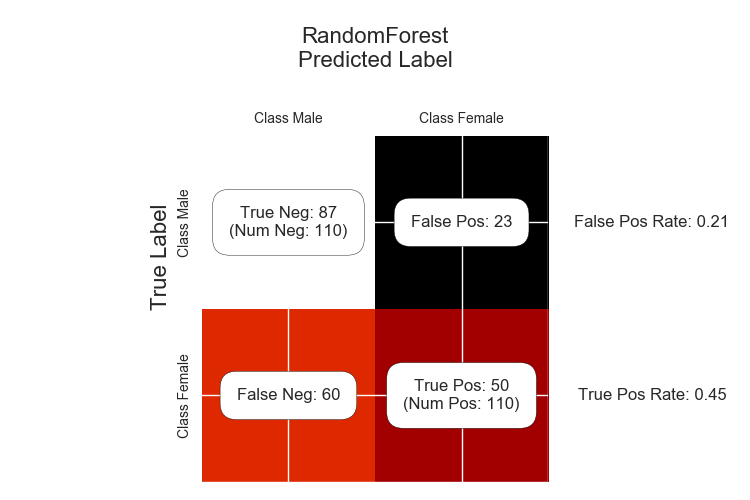
\includegraphics[width=0.5\textwidth]{figures/RandomForest}
    \label{RFCM}}
    \subfloat[Decision Tree]{%
    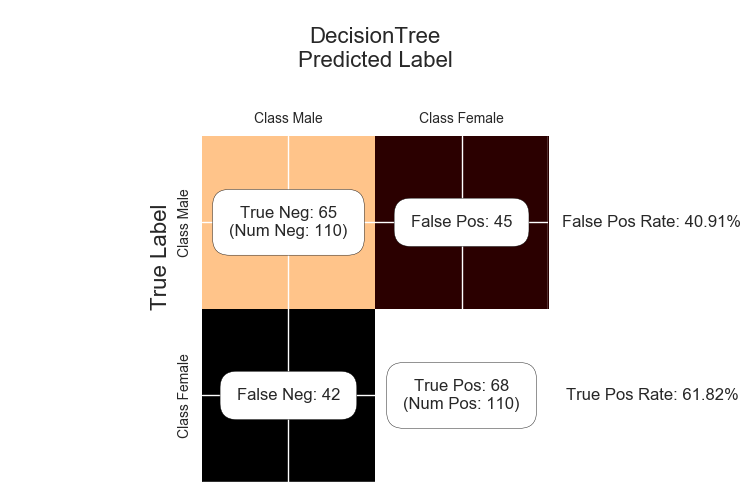
\includegraphics[width=0.5\textwidth]{figures/DecisionTree}
    \label{DTCM}}

    \quad


    \subfloat[XgBoost]{%
    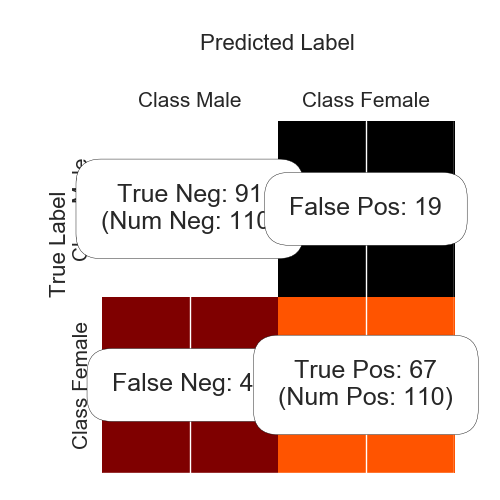
\includegraphics[width=0.5\textwidth]{figures/XGBoost}
    \label{XGBCM}}
    \subfloat[SVC]{%
    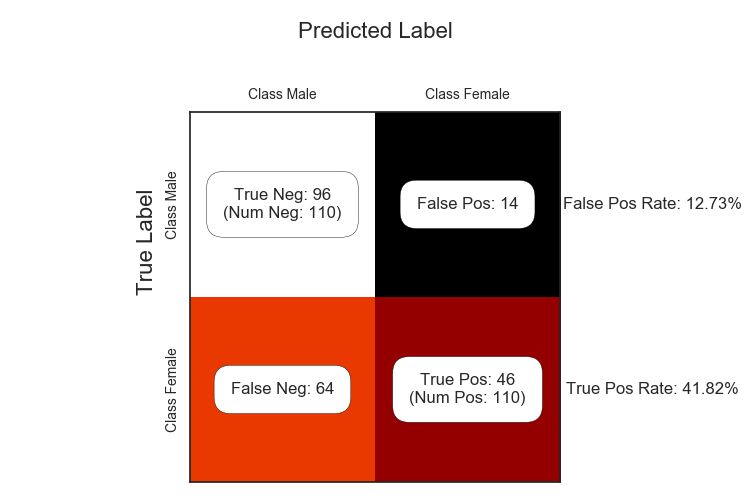
\includegraphics[width=0.5\textwidth]{figures/SVC}
    \label{SVCCM}}

    \caption{\textbf{Confusion Matrices of Baseline Classifiers}}
\end{figure}



%----------------------------------------------------------------------------------------
%  CHAPTER 
%----------------------------------------------------------------------------------------

\chapter*{Results}


\section*{Model Evaluation and Validation}

We tuned our model using sklearn's \texttt{GridSearch} in conjunction with a \{k=50 fold\} \texttt{StratifiedShuffleSplit} function, we tuned both the tree parameters as well as the task parameters of our XGBoost classifier to control for over-fitting and improve over all performance. The parameters we tuned are as follows:

\begin{itemize}
\item Parameters for Tree Booster
    \begin{itemize}
        \item \texttt{max\_depth}
        \begin{itemize}
            \item Maximum depth of tree
            \item Range [1, $\infty$], default 6, tuned on $[4, 6, 8, 10]$
        \end{itemize}
        \item \texttt{n\_estimators}
        \begin{itemize}
            \item Minimum number of trees
            \item Range $[2,\infty]$ default 2, tuned on $range(100, 1100, 100)$
        \end{itemize}

    \end{itemize}

\item Task Parameter
    \begin{itemize}
        \item \texttt{learning\_rate}
        \begin{itemize}
            \item Scale the contribution of each tree by learning rate
            \item Range $[0, 1]$, tuned on $[0.2222, 0.4444, 0.6666, 0.8888]$
        \end{itemize}
    \end{itemize}
\end{itemize}

Once we performed our search through the hyper-parameter space to find the combination of hyper-parameters that maximized the performance of our classifier, we were able to improve the previous $F_1$ score by 0.027\%. Here is the final model for classifying gender in introductory CS. 
\begin{verbatim}
XGBClassifier(base_score=0.5, colsample_bylevel=1, colsample_bytree=0.6,
       gamma=0, learning_rate=0.2222, max_delta_step=0, max_depth=6,
       min_child_weight=1, missing=nan, n_estimators=600, nthread=-1,
       objective='binary:logistic', reg_alpha=0, reg_lambda=1,
       scale_pos_weight=1, seed=0, silent=1, subsample=0.7)
\end{verbatim}

\begin{figure}[!hbtp]
\centering
    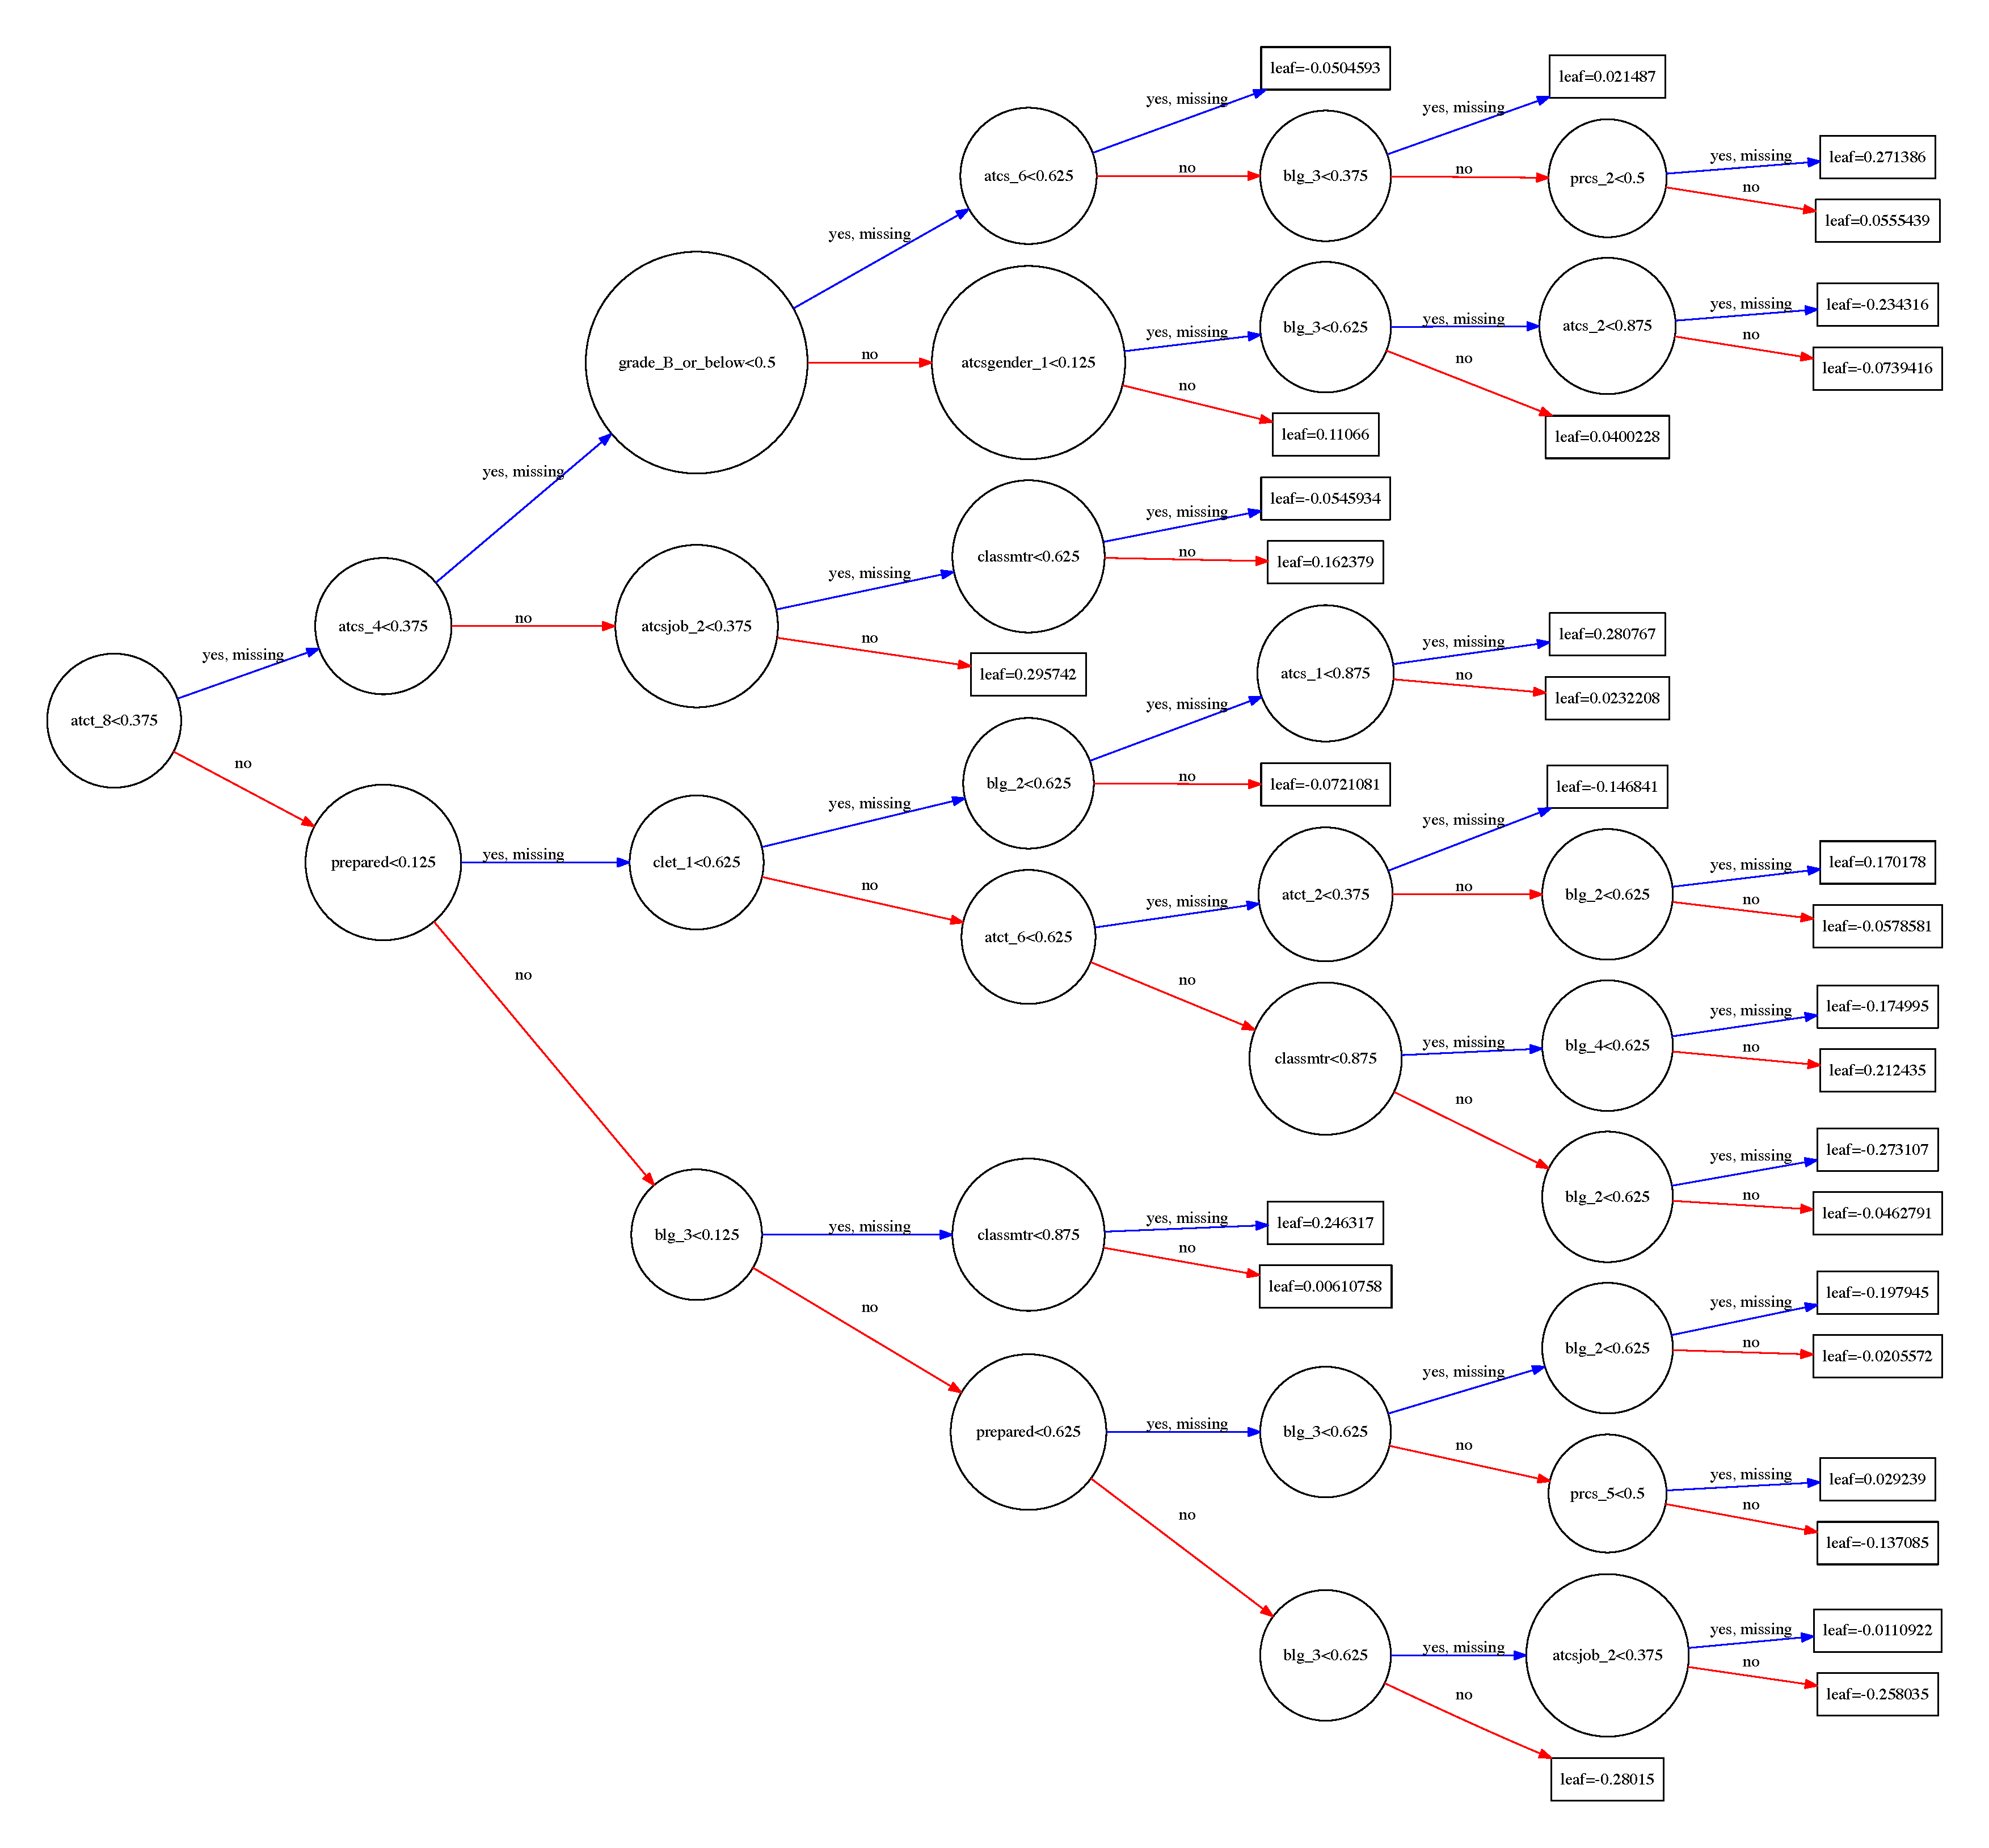
\includegraphics[width=1\textwidth]{figures/Tuned_model_graph}
    \caption{\textbf{Tuned XgBoost estimator decision tree. }\textit{}}\label{tuned_plot_tree}
\end{figure}

\begin{figure}[!hbtp]
\centering
    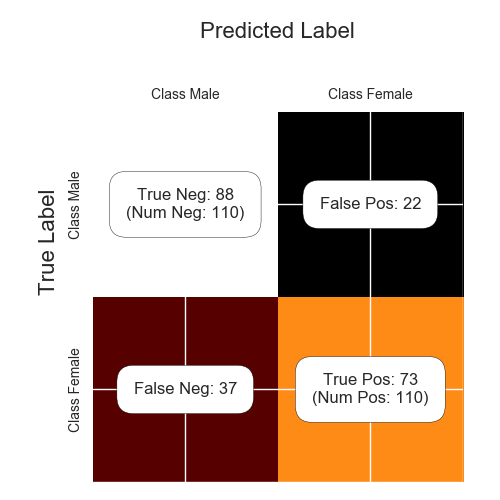
\includegraphics[width=0.8\textwidth]{figures/tuned_model_CM}
    \caption{\textbf{Tuned XgBoost model confusion matrix. }\textit{}}\label{tuned_CM}
\end{figure}

%----------------------------------------------------------------------------------------
%  CHAPTER 
%----------------------------------------------------------------------------------------

\chapter*{Conclusion}



\section*{Reflection}

